\section{Mockups}
\textbf{ Για τη δημιουργία των Mockups χρησιμοποιήθηκε το λογισμικό adobe photoshop }
\begin{figure}[!htb]
  \centering
    \centering
    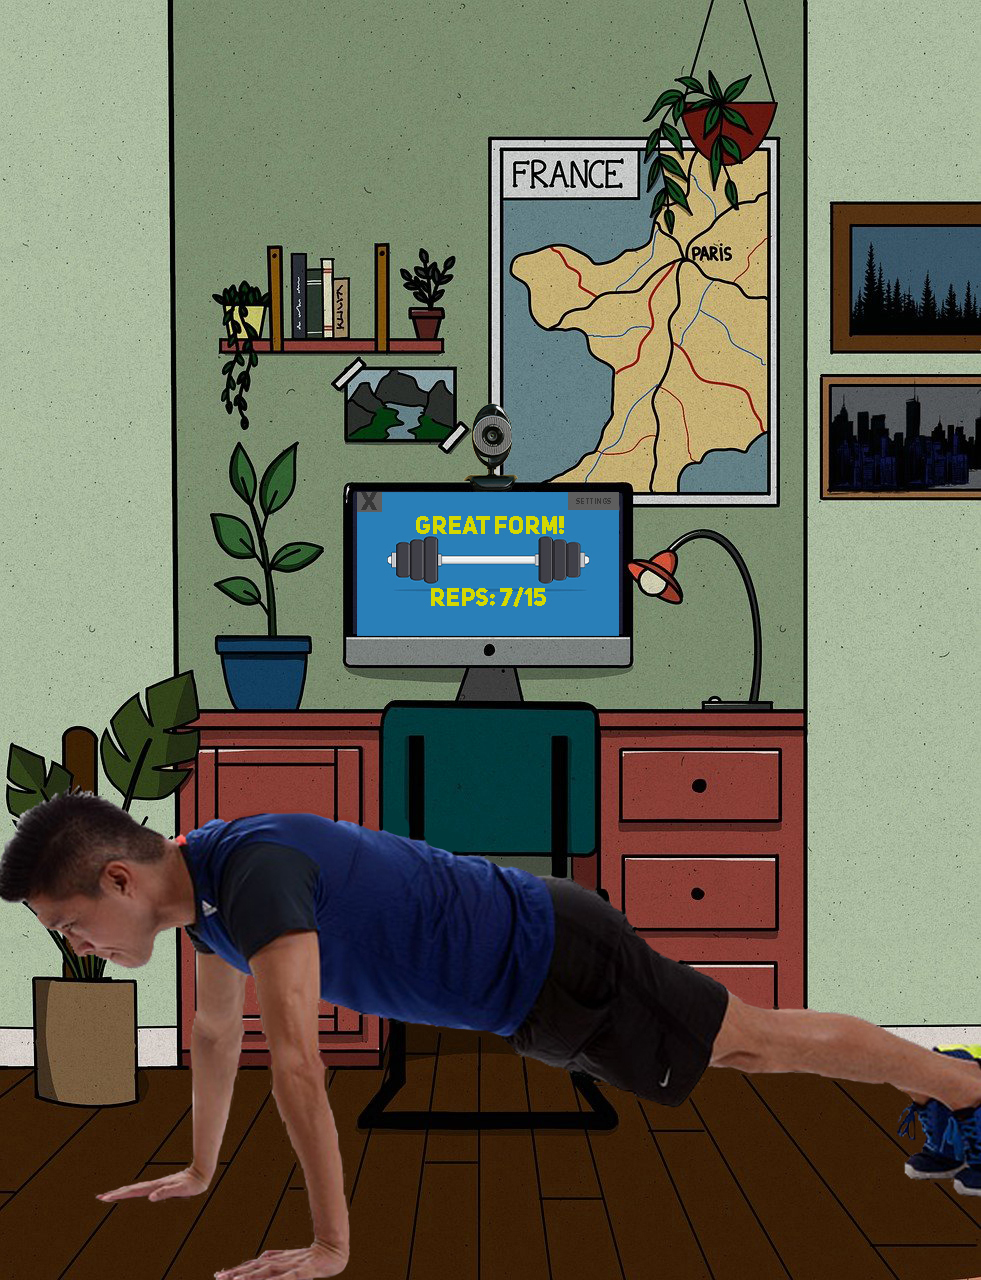
\includegraphics[width=\textwidth]{mockup1.jpg}
    \caption{Camera preview}
    \label{}
\end{figure}
\begin{figure}[!htb]
  \centering
    \centering
    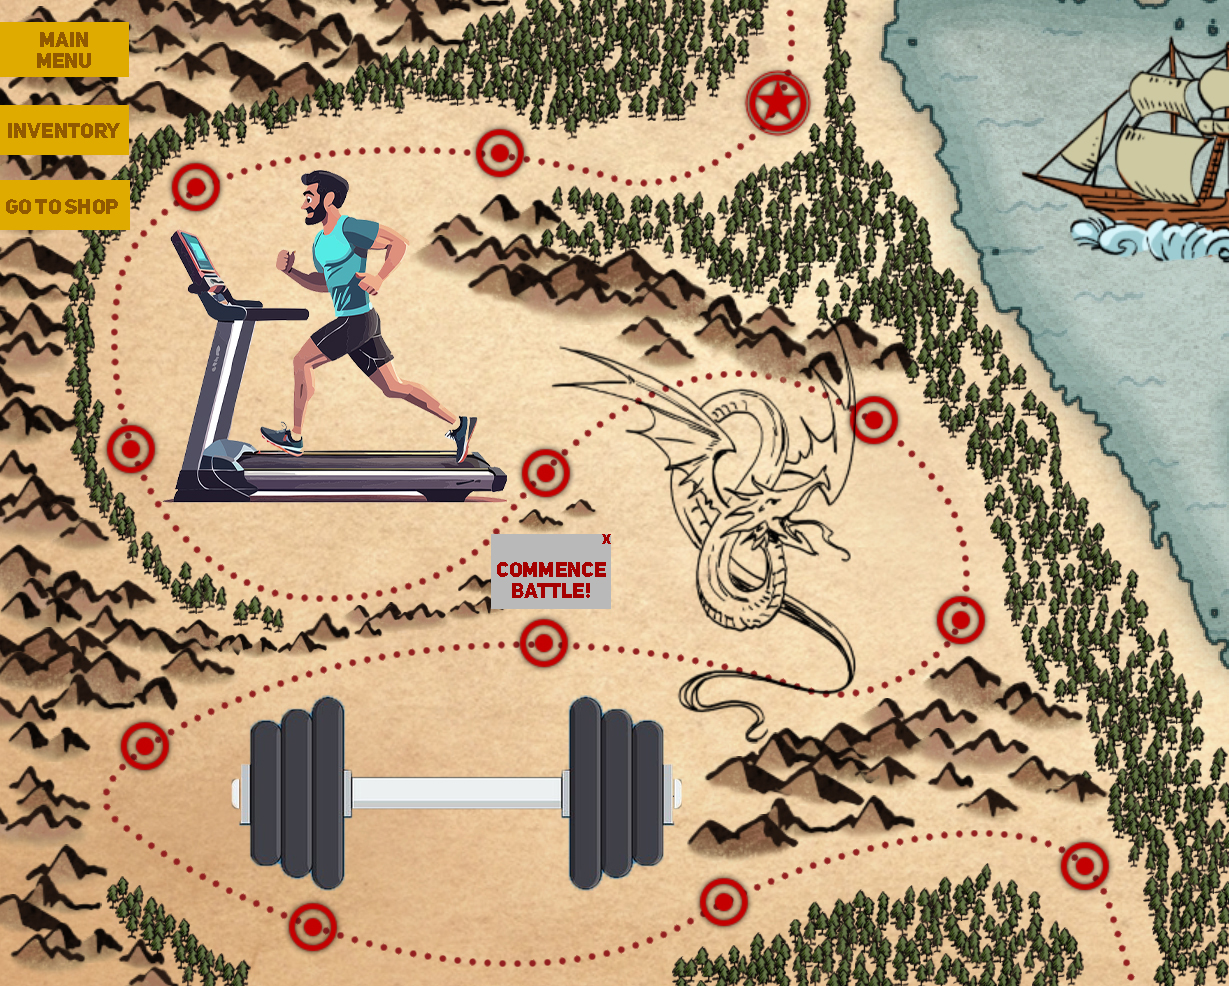
\includegraphics[width=\textwidth]{mockup2.jpg}
    \caption{Map preview}
    \label{}
\end{figure}
\begin{figure}[!htb]
  \centering
    \centering
    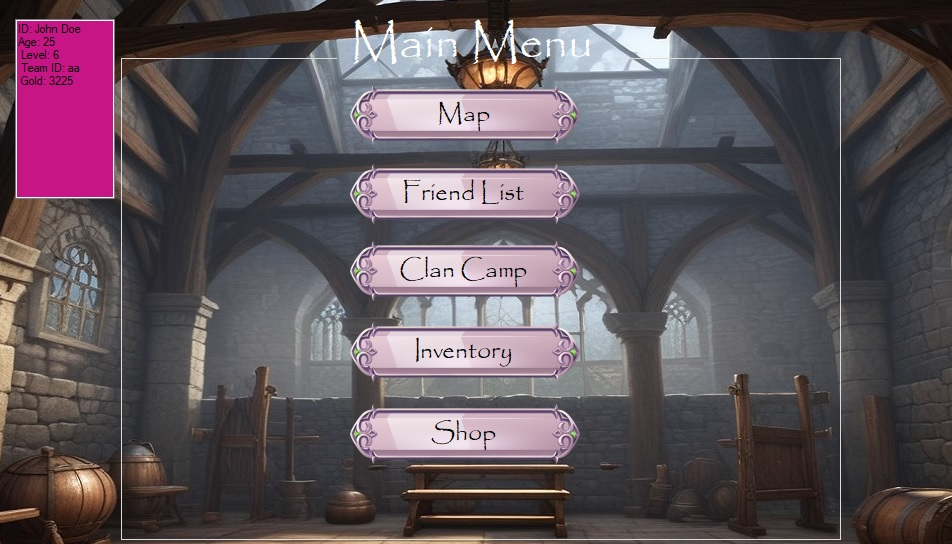
\includegraphics[width=\textwidth]{mockup3.jpg}
    \caption{Main menu}
    \label{}
\end{figure}
\begin{figure}[!htb]
  \centering
    \centering
    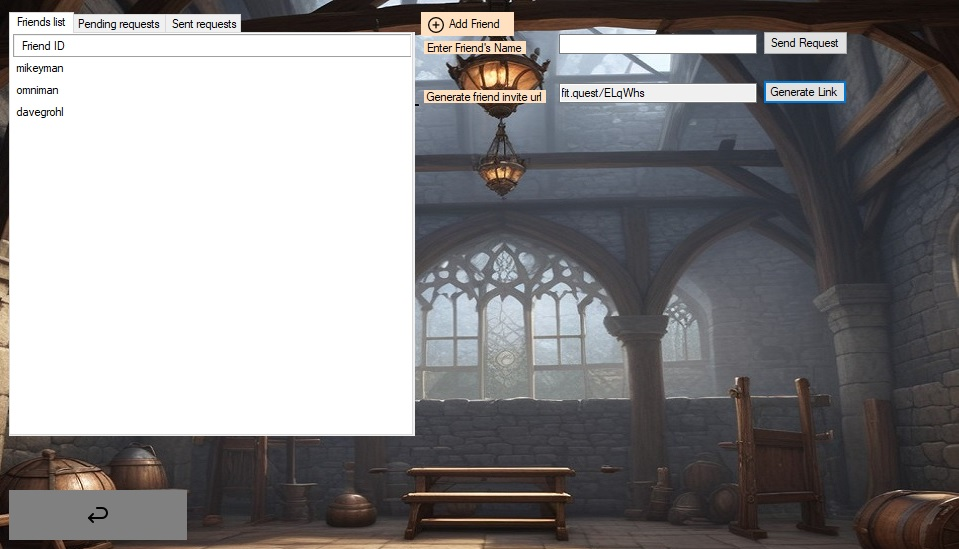
\includegraphics[width=\textwidth]{mockup4.jpg}
    \caption{Friends list}
    \label{}
\end{figure}
\begin{figure}[!htb]
  \centering
    \centering
    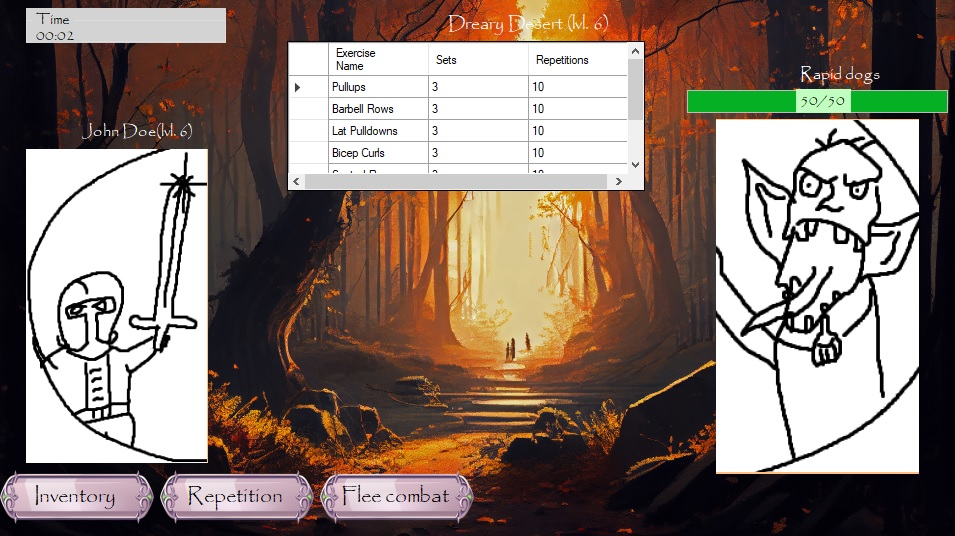
\includegraphics[width=\textwidth]{mockup5.jpg}
    \caption{Solo combat}
    \label{}
\end{figure}
\begin{figure}[!htb]
  \centering
    \centering
    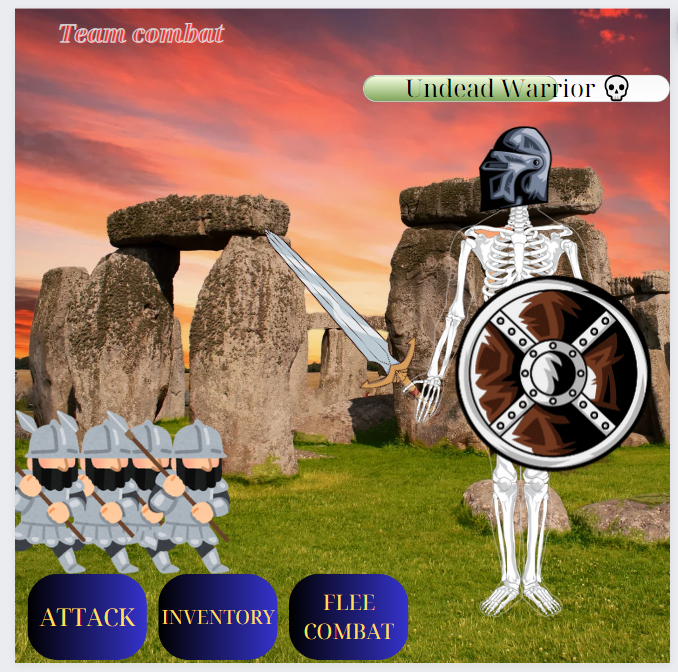
\includegraphics[width=\textwidth]{mockup6.jpg}
    \caption{Clan combat}
    \label{}
\end{figure}
\begin{figure}[!htb]
  \centering
    \centering
    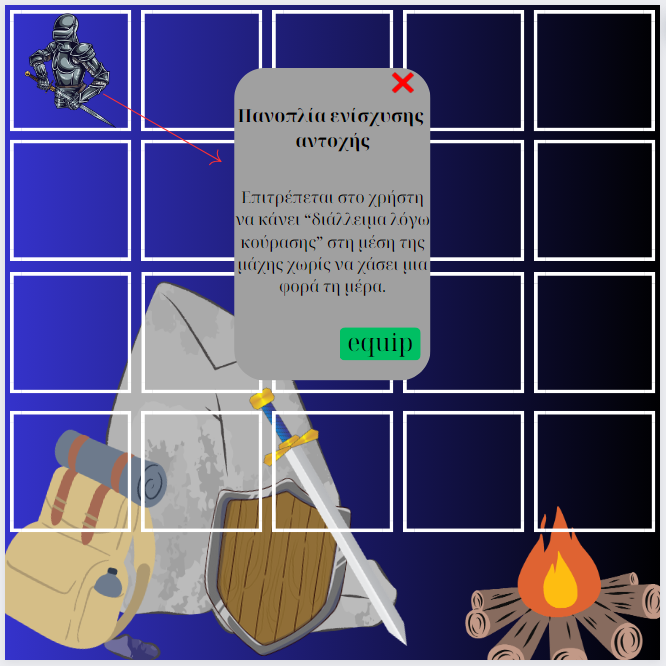
\includegraphics[width=\textwidth]{mockup7.jpg}
    \caption{Inventory}
    \label{}
\end{figure}
\begin{figure}[!htb]
  \centering
    \centering
    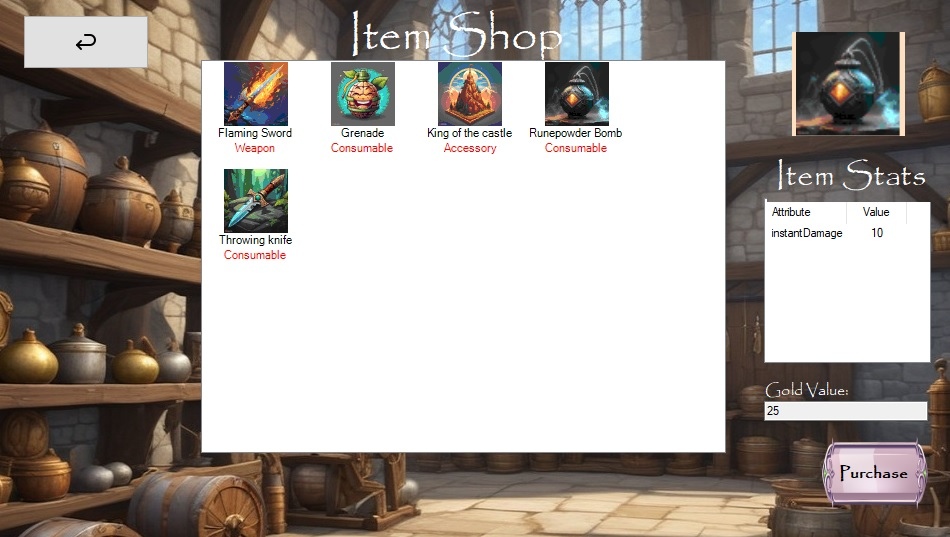
\includegraphics[width=\textwidth]{mockup8.jpg}
    \caption{Shop}
    \label{}
\end{figure}	
\begin{figure}[!htb]
  \centering
    \centering
    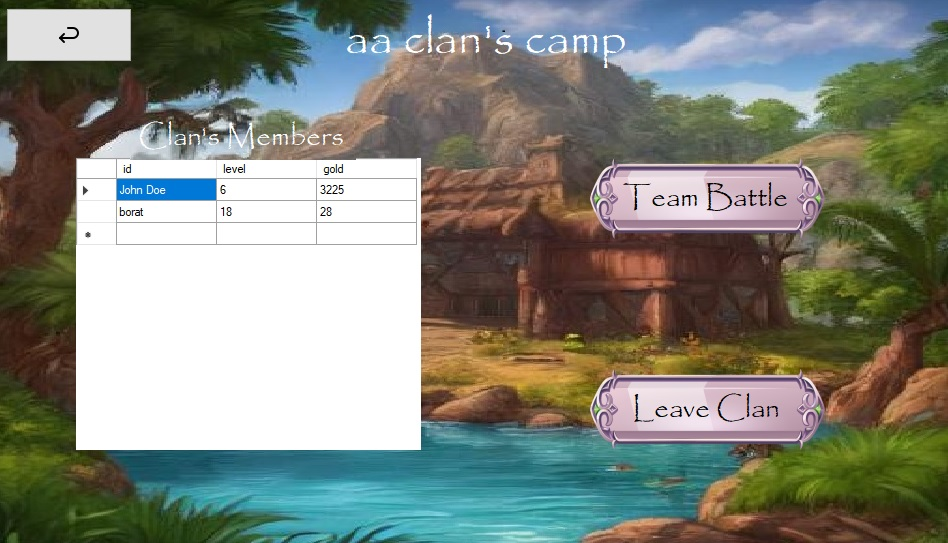
\includegraphics[width=\textwidth]{mockup9.jpg}
    \caption{Clan camp}
    \label{}
\end{figure}